\newpage
\section{Theoretische Grundlagen}
\label{sec:grundlagen}
%zugrundeliegende Theorien und Modelle
% Definitionen
% Stand der Technik, Normen und Standards, Wirtschaftliche Aspekte
% persönliche Positionierung


\todo[inline]{Optional Stand der Technik betrachten --> Fassfolgeplatten Systeme}

\subsection{Chemische Produktion und Prozesssicherheit}
Es gibt verschiedene Charakteristika, die den Betrieb einer chemischen Anlage beschreiben. Dazu gehören zum einen die technische Ausführung der Verfahrenstechnik, aber auch Aspekte wie die Arbeitsweise der Produktion oder das vorliegende Sicherheitskonzept.

\subsubsection{Produktionsweisen in der Chemie}
Chemieanlagen können je nach Produkt und Produktionsmenge auf verschiedene Weisen produzieren. 

\paragraph{Batch-Betrieb} Eine Arbeitsweise der chemischen Produktion stellt der sogenannte Batch-Betrieb, auch Chargenbetrieb genannt, dar. Bei dieser Fahrweise werden jegliche Prozess- und Verfahrensschritte in zeitlich festgelegter Reihenfolge nacheinander durchgeführt. Die Ausgangsstoffe werden hierfür in ein geeignetes Reaktionsgefäß, wie zum Beispiel einen Rührkessel, gegeben und die Reaktion gestartet. Danach wird das Reaktionsprodukt in entsprechende Lagertanks oder Gebinde transferiert und das Reaktionsgefäß gereinigt.\linebreak
Gerade für geringe Produktionsmengen oder häufigerem Wechsel der Produkte wird diese Betriebsweise bevorzugt. Durch den variablen Aufbau der Anlage werden somit auch verschiedene Reaktionszeiten und Herstellungsverfahren möglich gemacht.\,\cite{Ignatowitz.2015}\linebreak
In der Produktionsplanung einer solchen Produktionsweise können mehrerer Batches auf einer Fertigungslinie für das selbe Produkt geplant werden. Die Zusammenfassung dieser Batches wird allgemein als Produktionskampagne bezeichnet und hat den Vorteil, dass mehrere Batches hintereinander gefahren werden und somit weniger Unterbrechungen durch mögliche Umrüst- oder Reinigungsarbeiten entstehen. Zudem lassen sich bei der Lagerung einer Kampagne durch die einzelnen Batches Produktionsabweichungen ausgleichen.\,\cite{SAP.04.02.2022}

\paragraph{Kontinuierlicher Betrieb} Dem Batch-Betrieb gegenüber steht der kontinuierliche Betrieb. Im Gegensatz zur zeitlichen Taktung von Batch-Anlagen findet für diese Arbeitsweise eine örtliche Separierung der Verfahrensschritte bei kontinuierlichem Massenstrom statt. Die Prozessbedingungen, wie Temperatur, Druck oder Produktzusammensetzung sind deshalb stationär. Durch den festen Reaktionsablauf der Anlage eignet sich diese Fahrweise hauptsächlich für große Produktionsmengen. Neben dem Hauptprodukt fallen für diese Produktionsweise natürlich auch mögliche Nebenprodukte kontinuierlich an und sind entsprechend zu verwerten. \cite{Ignatowitz.2015}


\subsubsection{Industrielle Gebinde für Flüssigkeiten}
Um ein Edukt neu in die Produktion einzubinden sind, nicht nur die chemisch-physikalischen Eigenschaften relevant. Auch der Aspekt der Gebindeform ist maßgeblich für die Einfügung des Eduktes in den Produktionsablauf. Für flüssige Edukte sind im Tagesgeschäft der \textsc{Alberdingk Boley Leuna GmbH} hauptsächlich Kunststoff-IBCs (Intermediate Bulk Container) und zum Teil Kunststoff-Deckelfässer im Einsatz. Es sei jedoch erwähnt, dass auch weitere Gebinde auf dem Verpackungsmarkt verfügbar sind, wie beispielsweise Flüssig-IBCs, Kanister, Hobbocks oder Metallfässer.\\
Den IBC als kubisches Gebinde gibt ca. seit den 1960er Jahren  und hat sich über eine Richtlinie des VDI aus den frühen 70er-Jahren zu einem Standard der großen Einzelverpackungen entwickelt. Zuvor waren zum Großteil \SI{200}{\liter}-Fässer im Einsatz, welche sich neben der geometrischen Form auch maßgeblich im Handling zum IBC unterscheiden. \cite{neueverpackung.01.02.2022}
So lassen sich Fässer in dieser Größenordnung beispielsweise vorwiegend als 4er-Packung sicher transportieren und benötigen hierfür zusätzliche Paletten, sowie Schrumpffolie oder Transportbänder um die Behälter zu fixieren. Ein IBC hingegen kann direkt als Gebinde mit einem Hubwagen oder Gabelstapler transportiert werden ohne umfangreiche Vorbereitung. Weitere Punkte im Vergleich zwischen IBC und Fass finden sich unter Tabelle \ref{tab:ibc_fass}.

% Table generated by Excel2LaTeX from sheet 'Daten'
\begin{table}[h!]
	\renewcommand*{\arraystretch}{1.2}
	\centering
	%\rowcolors{2}{white}{gray!25}
	\caption{Allgemeiner Vergleich der Gebinde IBC und Fass \cite{MakrusKamroth.01.02.2022}}
	\label{tab:ibc_fass}
	\resizebox{\textwidth}{!}{
		\begin{tabulary}{1.0\textwidth}{C|C|C|C}
			\hline
			\textbf{} 						& \textbf{Einzelfass (1 Fass)} 			& \textbf{Fasspalette \linebreak (4 bis 5 Fässer)} & \textbf{IBC \linebreak (1 Container)}\\
			\hline
			\textbf{UN-Zertifikat} 		&	\multicolumn{3}{c}{möglich} \\
			\hline
			\textbf{Transportvorbereitung} 	& \multicolumn{2}{c|}{\parbox{6cm}{\centering \, \newline evtl. extra Palette mit Schrumpffolie/Transportbänder}}  & \parbox{3cm}{\centering \, \newline keine}\\
			\hline
			\textbf{Transport \linebreak (voll)} 				& schwer \linebreak mit Fassheber 	&\multicolumn{2}{c}{\parbox{6cm}{\centering \, \vspace*{2mm} \newline Gabelstapler, Flurförderzeuge}}\\
			\hline
			\textbf{Transport \linebreak (teilentleert)} 		& schwer \linebreak mit Fassheber 	& schwer mit Gabelstapler, Flurförderzeuge & Gabelstapler, Flurförderzeuge\\
			\hline
			\textbf{Abfüllmenge} 			& klein							& klein bis mittel				& mittel bis groß \\
			\hline
			\textbf{Lagerkapazität} 		& sehr klein			& klein	bis mittel				& groß\\
			\hline
			\parbox{3cm}{\, \vspace*{2mm} \newline \textbf{Erwärmbarkeit}}			& \parbox{2cm}{\centering \, \vspace*{2mm} \newline möglich}	 & \parbox{4cm}{\centering\, \vspace*{2mm} \newline nicht möglich}	 & möglich, \linebreak aber nicht effektiv\\
			\hline
			\textbf{Verwendung} 			& \multicolumn{2}{c|}{i.d.R einmalig} & mehrmals möglich\\
			\hline
			\textbf{Stapelbarkeit} 			& \multicolumn{2}{c|}{schlecht stapelbar} & gut stapelbar\\
			\hline
			\textbf{Produktreste} 		& \multicolumn{2}{c|}{$>\SI{5}{\kg}$}&$\leq\SI{5}{\kg}$\\
			\hline	
			\textbf{Anschlüsse} 		& \multicolumn{2}{c|}{Deckel oder Spundloch} & Deckel oder Auslaufarmatur	\\
			\hline
		\end{tabulary}
	}
\end{table}%
\FloatBarrier

\subsubsection{Sicherheit von Chemieanlagen}
Das Thema Sicherheit findet sich neben dem Gefahrguttransport in der Logistik natürlich auch im restlichen Umfang der Chemieanlage wieder. 
Vom Betreiber einer solchen Anlage ist durch verschiedene Gesetzte, Verordnungen und technischen Regeln ein Gesamtsicherheitskonzept zu erarbeiten und umzusetzen. Beispiele solcher Gesetze sind das Arbeitsschutzgesetzt, das Chemikaliengesetz, das Umweltverträglichkeitsgesetz und das Geräte- und Produktionssicherheitsgesetz GSPG. \linebreak 
Diese Gesetze münden dann seit dem Jahr 2002 in die Betriebssicherheitsverordung (kurz: BetrSichV), welche eine Gesamtbetriebssicherheitsverordnung darstellt und die eben genannten Gesetzte zusammenfasst. Weitere zu beachtende Verordnungen sind die Explosionsschutz- und die Gefahrstoffverordnung.\linebreak
Aus diesen Verordnungen setzten sich nun wiederum verschiedenste technische Regeln wie die EU-Richtlinie 94/9/EG (ATEX 100a), Technische Regeln für Behälter (TRB) oder Technische Regeln für Rohrleitungsanlagen (TRR) zusammen. Diese erleichtern das Umsetzen, der geforderten Verordnungen und Gesetze und bilden zusammen mit berufsgenossenschaftlichen Regelungen ein Gesamt-Sicherheitskonzept für eine chemische Anlage. \cite{Ignatowitz.2015}\\
Ausführung eines solchen Sicherheitskonzeptes in der Praxis zeigt sich zum Beispiel in Form von Arbeits- und Betriebsanweisungen für die Mitarbeiter. Aber auch regelmäßige Sicherheitsschulungen, Instandhaltung der Anlage, Nutzung sicherheitstechnischer Ausrüstung, Dimensionierung und Ausführung der Verfahrenstechnik, Ausweisung von Explosionszonen und viele weitere Punkte ergeben sich aus diesem festgelegten Sicherheitskonzept. Für weiterführende Informationen sei an dieser Stelle auf die angegebenen Verordnungen verwiesen. Für einen Überblick über die Thematik lassen sich weitere Informationen in \cite{Ignatowitz.2015} finden.

\paragraph{Zoneneinteilung explosionsgefährdeter Bereiche gemäß EU-Richtlinie 1999/92/EG}
Da das Sicherheitskonzept der \textsc{Alberdingk Boley Leuna GmbH} ebenfalls die Einteilung von Explosionszonen beinhaltet, wird die EU-Richtlinie 1999/92/EG (ATEX 137) in kurzer Form näher erläutert.Die Prüfung eines Bereiches auf eine explosionsgefährdete Zone erfolgt durch eine sicherheitstechnische Fachkraft in einem Explosionsschutzdokument. Wird der Bereich als explosionsgefährdet eingestuft, ist für Atmosphären aus brennbaren Gasen, Nebeln oder Dämpfen und Luft eine Festlegung auf die Zone 0, Zone 1 oder Zone 2 möglich. Diese unterscheiden sich nach Ausmaß der Explosionsgefährdung in diesem Bereich. Analog dazu teilen sich die Zonen 20, 21 und 22 in explosionsgefährdete Bereich für Staubwolken ein.\linebreak
In der EU-Richtlinie 1999/92/EG stellt Zone 2 der explosionsgefährdeten Bereiche den Bereich mit der geringsten Explosionsgefahr da. Im Normalbetrieb ist nicht davon auszugehen, dass eine explosionsfähige Atmosphäre entsteht und wenn dann nur kurzzeitig in Erscheinung tritt. Beispiele hiefür können Produktionsbereiche sein in denen mit brennbaren Flüssigkeiten hantiert wird. Zudem gehören Bereiche, welche die Zonen 1 und 0 näher umgeben ebenfalls zur Zone 2.\linebreak
Die Zone 1 beschreibt den nächsthöheren Grad der explosionsgefährdeten Bereiche. In dieser Zone treten im Normalbetrieb gelegentlich explosionsfähige Atmosphären als Gemisch aus brennbaren Gasen, Dämpfen oder Nebeln und Luft auf. Zu dieser Zone gehören jegliche Bereiche in nähere Umgebung zu Zone 0, aber auch zum Teil das innere von Reaktionsgefäßen, der nähere Bereich von leicht zerbrechlichen Armaturen (z.B. aus Glas) oder der Raum um Beschickungsöffnungen und Abfüllanlagen.\linebreak
Bereiche mit der größten Explosionsgefährdung werden mit Zone 0 gekennzeichnet. Hier sind explosionsfähige Atmosphären aus Luft und brennbaren Stoffen (Gase, Nebel, Dämpfe) häufig oder über längere Zeiträume vorzufinden. Meist werden die Bedingungen für diese Zone nur im Inneren von Behältern, Rohrleitungen oder Anlagen bedient.\,\cite{Ignatowitz.2015,bgn.2018}

\paragraph{Verwendung von Betriebsmitteln in Ex-Zonen gemäß EU-Richtlinie 2014/34/EU}
Möchte man nun ein neues Betriebsmittel, wie beispielsweise eine Pumpe, in der Anlage einführen ist hier ebenfalls der Explosionsschutz zu beachten. Hierfür gibt die EU-Richtlinie 2014/34/EU eine umfangreiche Möglichkeit der Einstufung und Kennzeichnung vor.
Neben einer Prüfung der Zündtemperatur für den verwendeten Prozessstoff sind für elektrische Betriebsmittel die Oberflächentemperaturen entscheidend für die Wahl der Temperaturklasse in Tabelle \ref{tab:temperaturklasse}. Die Zündtemperatur des Prozessstoffes sollte dabei mindestens \SI{40}{\celsius} über der zulässigen Oberflächentemperatur des Betriebsmittels sein. Die Angabe der Explosionszone und der Temperaturklasse sind als Minimum der zu tätigenden Einstufungen zu verstehen, um ein Betriebsmittel für einen explosionsgefährdeten Bereich auszulegen. Es sind jedoch auch weitere Aspekte und Einstufungen in der Richtlinie beschrieben, wie der Einsatzbereich, die Explosionsgruppe oder das Geräteschutzniveau, welche ebenfalls hinzugezogen werden sollten. Mehr dazu in einem sehr anschaulichen Plakat unter \cite{ECOM.2016} oder in \cite{bgci.10.02.2022}. 
\vspace*{-5mm}

\begin{table}[h!]
	\renewcommand*{\arraystretch}{1.2}
	\centering
	\caption{Temperaturklassen laut EU-Richtlinie 2014/34/EU, erstellt nach \cite{Ignatowitz.2015}}
	\label{tab:temperaturklasse}
	%\resizebox{10.5cm}{!}{
		\begin{tabulary}{1.0\textwidth}{C|C|C}
			\hline
			\textbf{Temperaturklasse} & \textbf{Betriebsmittel Oberflächentemperatur} & \textbf{Prozessstoff Zündtemperatur}\\
			\hline
			T 1 & \SI{450}{\celsius} & $\geq \SI{450}{\celsius} \rightarrow \SI{490}{\celsius} $\\
			T 2 & \SI{300}{\celsius} & $\geq \SI{300}{\celsius} \rightarrow \SI{340}{\celsius}$\\
			T 3 & \SI{200}{\celsius} & $\geq \SI{200}{\celsius} \rightarrow \SI{240}{\celsius}$\\
			T 4 & \SI{135}{\celsius} & $\geq \SI{135}{\celsius} \rightarrow \SI{175}{\celsius}$\\
			T 5 & \SI{100}{\celsius} & $\geq \SI{100}{\celsius} \rightarrow \SI{140}{\celsius}$\\
			T 6 & \SI{85}{\celsius} & $\geq \, \, \SI{85}{\celsius} \rightarrow \SI{125}{\celsius}$\\
			\hline			
	\end{tabulary}
%}
\end{table}%
\FloatBarrier

Aufgrund der hohen Explosionsgefährdung sind deshalb in den Zonen 0 und 1 nur Geräte erlaubt, die explosionssicher sind. Ist ein Gerät mit dem Symbol\,\exsymbol\, gekennzeichnet, darf es in einen der entsprechenden Zonen verwendet werden, da durch die nach Prüfung vergebene Kennzeichnung eine Explosion in einer explosionsfähigen Atmosphäre ausschließt. Technisch wird dies zum Beispiel durch eine druckfeste Kapselung oder Eigensicherheit gewährleistet. In Zone 2 ist die Regelung hierfür nicht so streng. Hier reicht es wenn das Gerät schwadensicher ist und es beim kurzfristigen auftreten einer explosionsfähigen Atmosphäre über mindestens \SI{2}{\hour} nicht zu Explosion kommt. \cite{Ignatowitz.2015}

%Weiterhin sind folgende Punkte zu beachten
%\begin{itemize}
%	\item sicherheitstechnische Ausrüstung (z.B. Sicherheitsventile, Gasmessgeräte, ...) ist bereitzustellen und zu nutzen
%	\item Sicherstellung von Wissen über die genutzten Gefahrstoffe und Vorgänge, sowie deren Beherrschung
%	\item Verfahrenstechnik in der Anlage ist sicherheitstechnisch einwandfrei auszulegen und überprüfen zu lassen
%	\item die Anlagendimensionierung sollte den genutzten Betriebsbedingungen und Chemikalien entsprechen und mit Sicherheitszuschlägen versehen werden
%	\item Sicherheit ist durch Instandhaltung der Anlage zu gewährleisten
%	\item Es sind EMSR und PLT-System zur Überwachung und Meldung von Störfällen in der Anlage zu nutzen
%	\item die Anlage ist mit qualifiziertem Personal in ausreichender Anzahl zu fahren
%	\item das an und in der Anlage arbeitende Personal hat sich regelmäßigen Sicherheitsunterweisungen zu unterziehen
%\end{itemize}

\subsection{Definition und Gliederung zu Verdickungsmitteln}

In der Farben- und Putzindustrie werden Verdickungsmittel als rheologische Additive bezeichnet. Sie erhöhen die Viskosität von Flüssigkeiten und ändern somit ihre rheologischen Eigenschaften, welche die Auftragungs-, Fließ- und Verlaufseigenschaften von Farben und Putzen bestimmen. Verdickungsmittel kommen jedoch auch in der Lebensmittelchemie oder Pharmazie zum Einsatz. Je nach dem welche Anforderungen an das Verdickermittel gestellt werden, unterscheiden sich diese in ihrer Zusammensetzung (siehe Abb. \ref{fig:verdicker_einteilung}). \cite{Brock.2009}

\begin{figure}[h!]
	\centering
	\begin{forest}
		forked edges,
		for tree={draw,align=center,edge={-latex}}
		[Verdickungsmittel, for children={fit=band}
		[Anorganisch]
		[Organisch, for children={fit=band}
		[Niedermolekular]
		[Synthetisch]
		[Natürlich, for children={fit=band}
		[Natürlich (abgewandelt)]
		]	
		]	
		]
	\end{forest}	
	\caption{Einteilung von Verdickungsmitteln nach Zusammensetzung \cite{Brock.2009}}
	\label{fig:verdicker_einteilung}
\end{figure}
\FloatBarrier

Je nach Verdickungsmittel können verschiedene Effekte wie Gelbildung, Solvatation, Ausbildung von Netzstrukturen, Coulomb-Kräfte, Quellung und Wasserstoff- Brückenbindungen, sowie deren gegenseitige Einflussnahme die Erhöhung der Zähflüssigkeit bewirken. \cite{Brock.2009} \\
Betrachtet man speziell die sogenannten assoziativen Verdickungsmittel lassen sich diese den Gruppen der abgewandelten, natürlichen Verdicker und den synthetischen Verdickern zuordnen.  Sie spezifizieren sich gegenüber anderen Verdickertypen darin, dass sie neben hydrophilen Gruppen auch hydrophobe End- und Seitengruppen enthalten, welche dem Verdickungsmittel einen Tensidcharakter verleihen. Deshalb bestehen assoziative Verdicker unteranderem aus hydrophob modifizierten Polymerstrukturen (siehe Abb. \ref{fig:assoziativ_einteilung}).

\begin{figure}[h!]
	\centering
	\begin{forest}
		forked edges,
		for tree={draw,align=center,edge={-latex}}
		[Assoziativverdicker
		[hydrophob \\ modifizierte \\ Polyacrylate]
		[hydrophob \\ modifizierte \\ Celluloseether]
		[hydrophob \\ modifizierte \\ Polyether]
		[hydrophob \\ modifizierte \\ Polyacrylamide]
		[assoziative \\ Polyurethan-Verdicker]
		]
	\end{forest}	
	\caption{Einteilung von Assoziativ-Verdickern nach chemischer Struktur \cite{Brock.2009}}
	\label{fig:assoziativ_einteilung}
\end{figure}
\FloatBarrier
Diese strukturelle Eigenschaft der Assoziativ-Verdicker macht die Bildung von Micellen möglich und es treten neben der Quellung in der Wasserphase sogenannte "`Micellbrücken"' zwischen Latex-Teilchen der Bindemitteldisperion auf, welche eine zusätzlich Viskositätserhöhung bewirken. \cite{Brock.2009} \\
In Abbildung \ref{fig:struktur_puverdicker} ist eine schematische Struktur eines solchen assoziativen Polyurethan-Verdickers aufgeführt. Diese beispielhafte Struktur zeigt hydrophile, höher molekulare Polyethersegmente, welche über Urethan-Gruppen verbunden sind und durch hydrophobe Molekülgruppen verknüpft werden. \cite{Brock.2009}

\begin{figure}[h!]
	\centering
	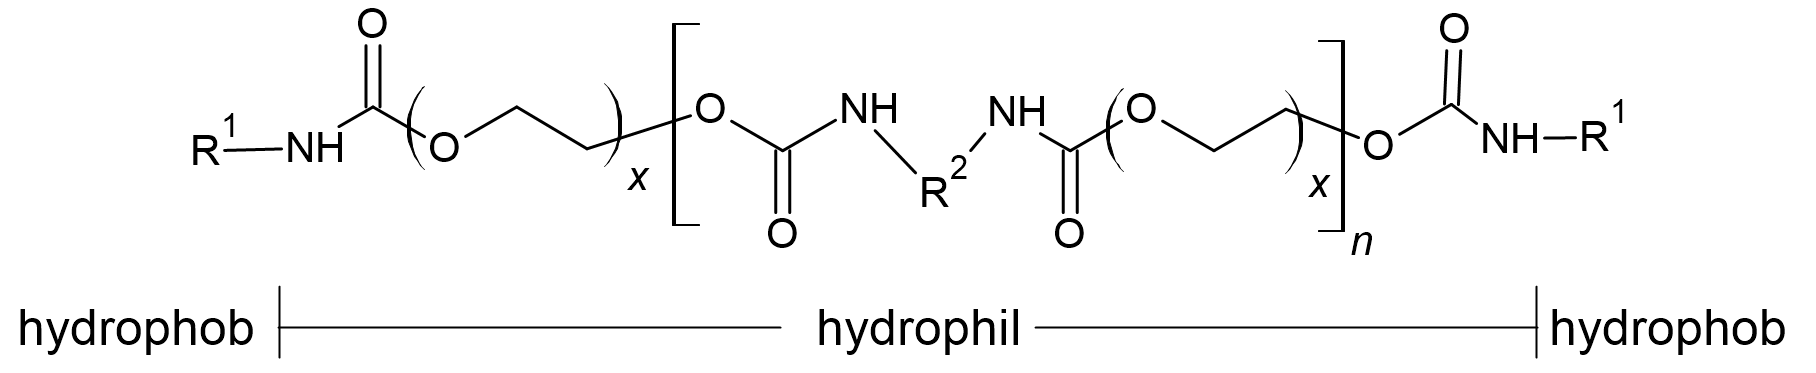
\includegraphics[width=0.75\textwidth]{img/verdicker_struktur}
	\caption{schematische Struktur eines assoziativen Polyurethan-Verdickers, \linebreak erstellt nach \cite{Brock.2009}}
	\label{fig:struktur_puverdicker}
\end{figure}
\FloatBarrier

Durch diesen Mix der hydrophoben und hydrophilen Strukturen wird der Tensidcharakter des Verdickungsmittels bestimmt und es ergeben sich Netzstrukturen mit assoziierten "`Micellbrücken"', wie in Abbildung \ref{fig: verdicker_anwendung} dargestellt. Zusätzlich ist zu erkennen, dass auch Wechselwirkungen mit bereits vorhandenen Tensidmolekülen in der Dispersion auftreten können und die Struktur somit weiter stabilisieren. \cite{Mezger.2016}

\begin{figure}[h!]
	\centering
	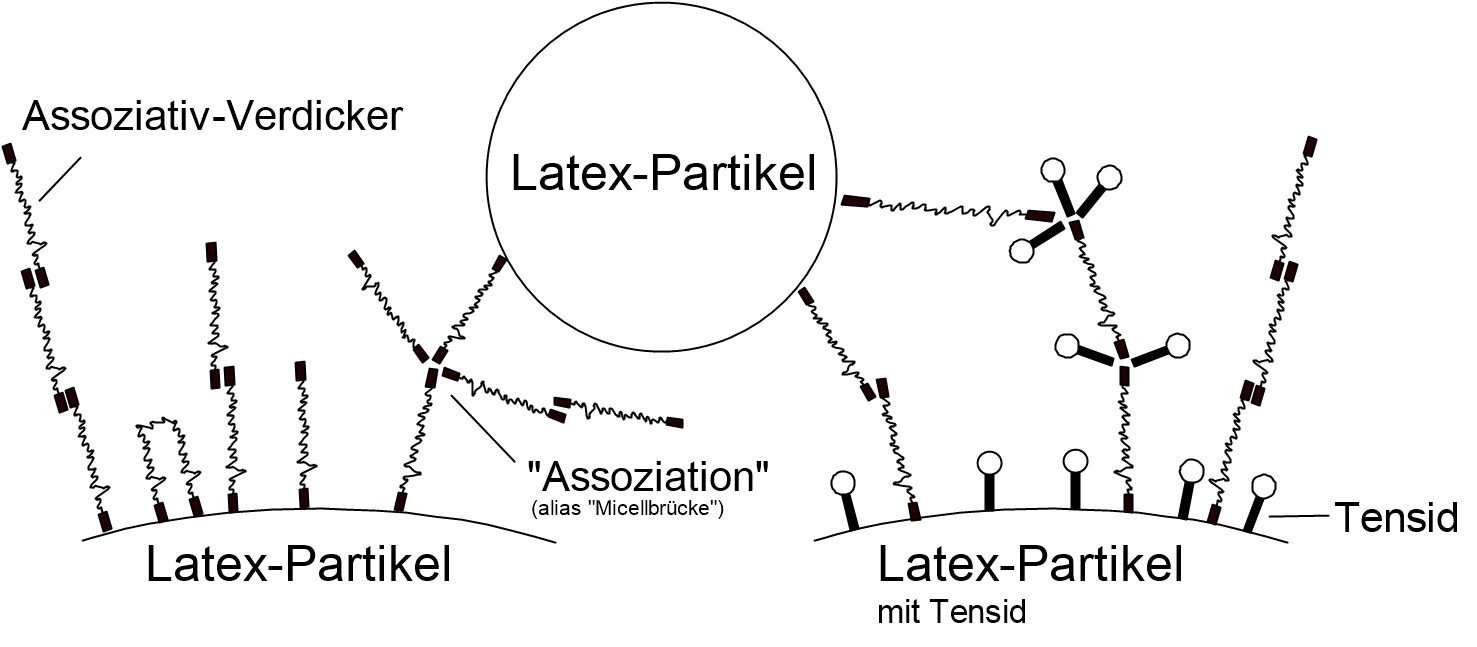
\includegraphics[width=0.75\textwidth]{img/verdicker_anwendung}
	\caption{Netzstruktur durch Verdickermittel in Latex-Dispersion (mit und ohne Tensid), \linebreak erstellt nach \cite{Mezger.2016}}
	\label{fig: verdicker_anwendung}
\end{figure}
\FloatBarrier

Aufgrund dieser ausgeprägten Netzstrukturen innerhalb des Verdickungsmittels ist es jedoch auch möglich, dass das Verdickungsmittel selbst eine hohe Viskosität aufweist. Dieser Punkt kann erheblichen Einfluss auf die großtechnische Verarbeitbarkeit des Additives haben und wird im weiteren Verlauf dieser Arbeit näher betrachtet. 

\subsection{Dosierung von Flüssigkeiten}

\subsubsection{Charakterisierung des Dosierstroms}
\paragraph*{Rheologie von Fluiden} Um den Dosierstrom einer Flüssigkeit charakterisieren,  ist es zunächst nötigt die Fließeigenschaften beschreiben zu können. Die Wissenschaft der Rheologie beschäftigt sich unter anderem mit dem Fließ- und Deformationsverhalten von Flüssigkeiten und teilt diese zunächst in \textsc{Newtonsche} und \textsc{Nichtnewtonsche} Fluide ein. Grundlage dieser Einteilung sind Untersuchungen von \textsc{Isaac Newton}, welcher sich bei konstanter Temperatur mit der Schergeschwindigkeit $D$ in Abhängigkeit von der Schubspannung $\tau$ beschäftigte. 
Das Ergebnis dieser Arbeit ist das \textsc{Newtonsche Fließgesetz} unter Gleichung \eqref{eq: newton}, welche den Fließwiderstand $\eta$ einer Flüssigkeit bei gegebener Temperatur als Stoffkonstante benennt. Dieser Fließwiderstand $\eta$ ist heute unter der Bezeichnung der dynamischen Viskosität bekannt.

\begin{equation}
	\label{eq: newton}
	\tau = \eta * D
\end{equation}
\begin{parameter}
	D 			& Schergeschwindigkeit\\
	\tau 		& Schubspannung\\
	\eta 		& Dynamische Viskosität\\
\end{parameter}

Es sei erwähnt, dass neben der dynamischen Viskosität auch eine kinematische Viskosität $\nu$ existiert. Diese beschreibt in Gleichung \eqref{eq:kivisko} jedoch lediglich das Verhältnis zwischen der dynamischen Viskosität und der Dichte eines Fluides.

\begin{equation}
	\label{eq:kivisko}
	\nu = \frac{\eta}{\rho}
\end{equation}
\begin{parameter}
	\nu 		& kinematische Viskosität\\
	\rho 		& Dichte\\
	\eta 		& Dynamische Viskosität\\
\end{parameter}

Schlussendlich gilt für die Einteilung der Fluide nach Gleichung \eqref{eq: newton}, dass alle Fluide, welche eine Linearität zwischen Schergeschwindigkeit und Schubspannung ohne Fließgrenze aufweisen als \textsc{Newtonsche} Fluide und diejenigen, die ein nicht-lineares Verhalten und/oder ein Verhalten mit Fließgrenze aufweisen als \textsc{Nichtnewtonsche} Fluide eingeordnet werden. Veranschaulicht wird dies in Abbildung\,\ref{fig: arten_fluide} mit einer Auswahl an verschiedenen Rheologieprofilen.

\begin{figure}[h!]
	\begin{minipage}[b]{0.475\textwidth}
		\centering
		\includegraphics[width=\textwidth]{img/fluidarten}
		\caption{Fließkurven für verschiedene \linebreak Fluide, erstellt nach \cite{Holze.2010}}
		\label{fig: arten_fluide}
	\end{minipage}
	\hspace*{0.05\textwidth}
	\begin{minipage}[b]{0.475\textwidth}
		\centering
		\includegraphics[width=\textwidth]{img/fluidarten2}
		\caption{Viskositätskurven für verschiedene Fluide, erstellt nach \cite{MunzingChemieGmbH.2018}}
		\label{fig: arten_fluide2}
	\end{minipage}
\end{figure}
\FloatBarrier

%\paragraph*{Messmethoden zur Viskositätsbestimmung}
Zur Bestimmung der Viskosität müssen für ein \textsc{Newtonsches} Fluid laut Gleichung\,\eqref{eq: newton} die Schergeschwindigkeit $D$ und die Schubspannung $\tau$ bestimmt werden. Eine Möglichkeit hierfür ist die Nutzung eines sogenannten Rotationsviskosimeters. Allgemein beschreiben Rotationsviskosimeter einen Viskosimetertypen, bei dem die zu messende Flüssigkeit zwischen spezifisch geformten Körpern gebracht wird, von denen einer rotiert. Dabei tritt eine Scherung der Flüssigkeit auf und das aufgewendete Drehmoment am Viskosimeter wird gemessen. Neben Rotationsviskosimetern sind auch weitere Viskosimetertypen wie Kappilarviskoskosimeter und Fallkörperviskosimeter bekannt. Diese unterscheiden sich neben dem Aufbau gegenüber dem Rotationsviskosimeter beispielsweise auch darin, dass sie im Regelfall die Viskosität von \textsc{Nichtnewtonschen} Fluiden nicht ausreichend untersucht werden kann. \cite{ROMPPRedaktion.2008}

\paragraph*{Bestimmung der Strömungsform} Nachdem die Viskosität bestimmt ist, lässt sich nun der Dosierstrom des Verdickermittels entsprechend seiner Strömungseigenschaften beschreiben. Hier für wird die sogenannte \textsc{Reynoldszahl} bestimmt. Sie ist eine dimensionslose Kennzahl und beschreibt das Verhältnis zwischen Trägheitskräften zu Reibungskräften in strömenden Flüssigkeiten und ist für durchströmte Rohrleitungen unter Gleichung\,\eqref{eq: reynolds} definiert. \cite{Foth.2014}

\begin{equation}
	\label{eq: reynolds}
	Re = \frac{d_H*\rho*\overline{u}}{\eta}
\end{equation}
\begin{parameter}
	Re 			& 	\textsc{Reynoldszahl} \\
	\eta 		& dynamische Viskosität des Fluids\\
	\rho 		& Dichte des Fluids\\
	d_H			&	hydraulischer Rohrdurchmesser\\
	\overline{u} & mittlere Strömungsgeschwindigkeit\\
\end{parameter}

Anhand der \textsc{Reynoldszahl} lässt sich nun mithilfe der Tabelle \ref{tab:stromung_reynolds}, die jeweilige Strömungsform zuordnen. Diese Zuordnung ist wichtig, da sich je nach Strömungsform unterschiedliche Einflussgrößen auf den Druckverlust somit auf die Auslegung der Dosierung ergeben. Beispielsweise hat für eine laminare Strömung die Wandrauigkeit der Leitung keinen Einfluss mehr, wohin gegen sie in turbulenten Strömungen maßgebliche Druckverluste hervorrufen kann. In laminaren Strömungen überwiegt hierbei der glättende Einfluss der Viskosität gegenüber den Rohrunebenheiten, während in turbulenten Strömungen weitere Wirbel erzeugt werden. \cite{Bschorer.2018}

% Table generated by Excel2LaTeX from sheet 'Daten'
\begin{table}[h!]
	\renewcommand*{\arraystretch}{1.2}
	\centering
	\caption{Strömungsformen und ihre Reynoldszahlen \cite{Foth.2014}}
	\label{tab:stromung_reynolds}
	%\resizebox{10.5cm}{!}{
		\begin{tabulary}{1.0\textwidth}{C|CCC}
			\hline
			\textbf{Strömungsform} & \textbf{Laminar} & \textbf{instabiler Bereich} & \textbf{Turbulent}\\
			\hline
			\textbf{Reynoldszahl} &	$< 2300$ & $2300$ bis $4000$& $>4000$\\
			\hline			
		\end{tabulary}
		%}
\end{table}%
\FloatBarrier

Nach der Bestimmung der Reynoldszahl lässt sich nun mit Hilfe des \linebreak \textsc{Nikuradse-Colebrook-Moody}-Diagramms, nachfolgend \textsc{Moody}-Diagramm genannt, die Rohrreibungszahl $\lambda$ bestimmen (siehe Abb. \ref{fig:moody}). Diese Rohrreibungszahl ist eine dimensionslose Kennzahl und kann zweckmäßig in Gleichung \eqref{eq:druckverlustbeiwert} eingesetzt werden. Somit ist es möglich den dimensionslosen Druckverlustbeiwert $\zeta_R$ für gerade Rohrleitungen zu bestimmen und ermöglicht daraufhin die Berechnung des durch Reibung verursachten Druckverlustes $\Delta p$ auf Basis der erweiterten \textsc{Bernoulli}-Gleichung \eqref{eq:druckverlust_zeta}. \cite{Bschorer.2018}

\begin{equation}
	\label{eq:druckverlustbeiwert}
	\zeta_R = \lambda * \frac{L}{d}
\end{equation}
\begin{equation}
	\label{eq:druckverlust_zeta}
	\Delta p = \frac{1}{2}*\zeta_R*\rho*\overline{u}^2
\end{equation}
\begin{parameter}
	\zeta_R		& Druckverlustbeiwert für gerade Rohrstrecken\\
	L 			& Rohrleitungslänge\\
	d			& Rohrdurchmesser\\
	\Delta p	& Druckverlust \\
	\rho 			& Dichte des Fluids\\
	\overline{u} 	& mittlere Strömungsgeschwindigkeit\\
\end{parameter}


\begin{figure}[h!]
	\centering
	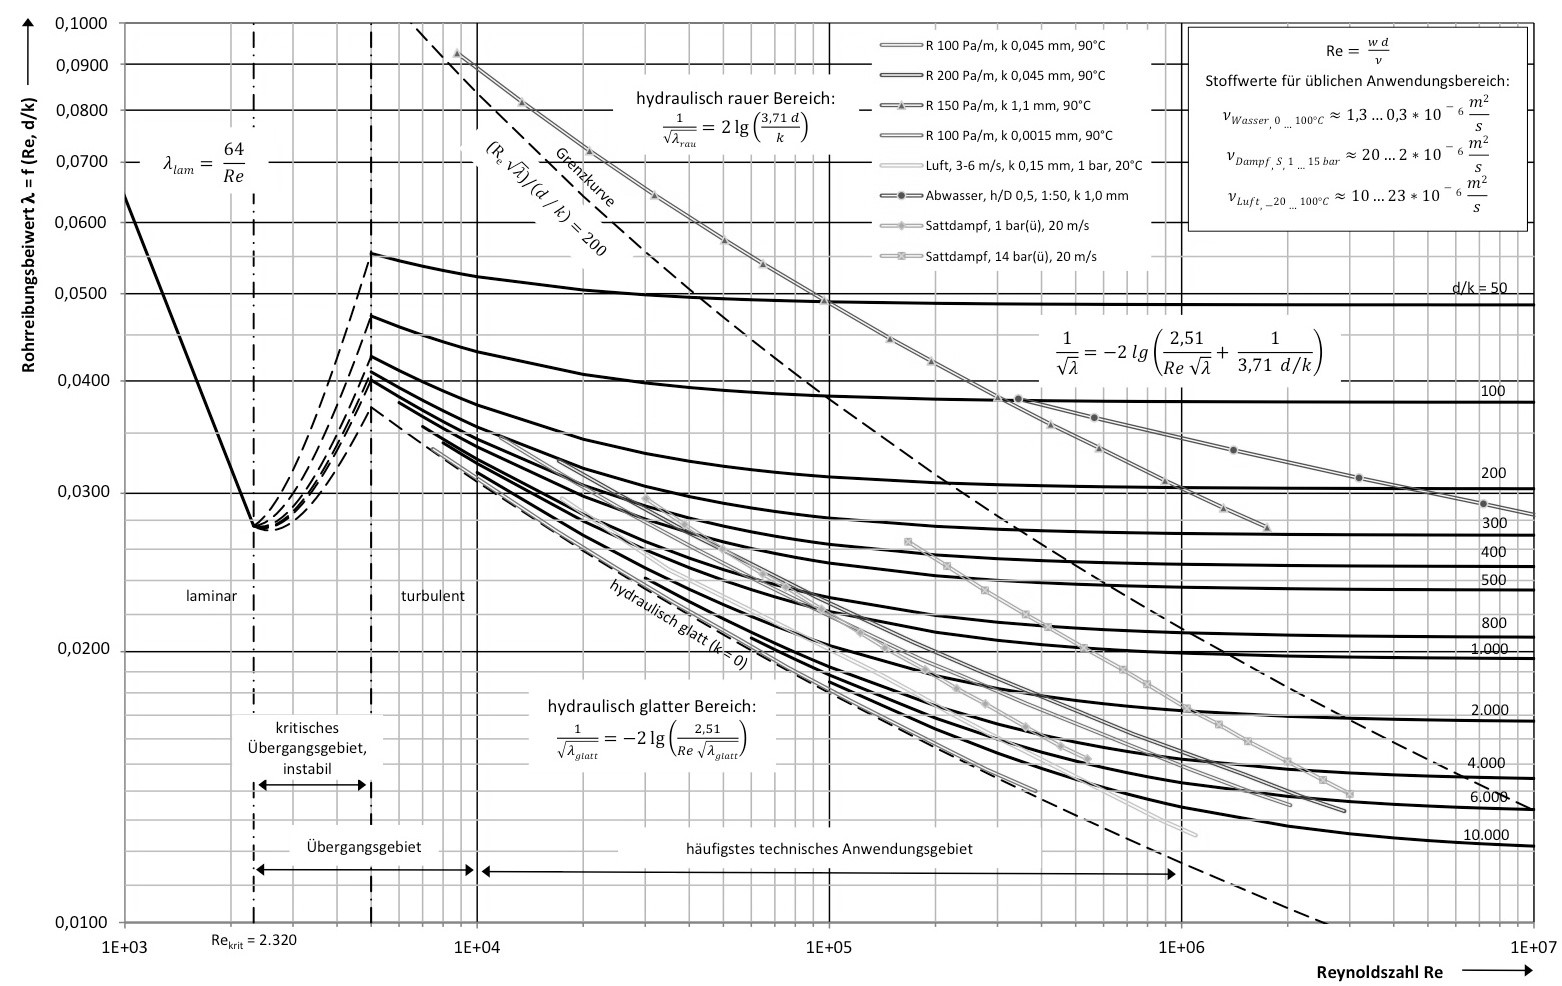
\includegraphics[width=1.0\textwidth]{img/R_Rohrreibungsbeiwert.jpg}
	\caption{\textsc{Nikuradse-Colebrook-Moody}-Diagramm \cite[\ccbysa]{Msimca.2017}}
	\label{fig:moody}
\end{figure}
\FloatBarrier
%Ende

\paragraph*{Gesetz von  \textsc{Hagen}-\textsc{Poiseuille}} Liegt für eine nicht-kompressible Flüssigkeit eine laminare Strömung vor, so ist es möglich die zuvor beschriebene Vorgehensweise zu vereinfachen und den auftretenden Druckverlust in einer geraden Rohrleitung direkt mit dem Gesetz von \textsc{Hagen}-\textsc{Poiseuille} zu bestimmen.  Der Druckverlust wird hierbei in Abhängigkeit vom Volumenstrom, der Rohrleitungslänge, des Rohrdurchmessers und der Viskosität berechnet. Die Definition des Gesetzes, aufgelöst nach dem Druckverlust, findet sich unter Gleichung \eqref{eq:hagen}. \cite{Foth.2005}

\begin{equation}
	\label{eq:hagen}
	\Delta p  = \frac{8*\eta*L*\dot{V}}{r^4*\pi}
\end{equation}
\begin{parameter}
	\Delta p	& Druckverlust \\
	\eta 		& dynamische Viskosität des Fluids\\
	\dot{V}		& Volumenstrom des Fluids\\
	r			& innerer Radius der Rohrleitung\\
	L 			& Rohrleitungslänge\\
\end{parameter}

Da das Gesetz von \textsc{Hagen}-\textsc{Poiseuille} bereits im \textsc{Moody}-Diagramm enthalten ist, können beide Vorgehensweisen genutzt werden um die jeweils andere Rechnung zu überprüfen. Sollen Rohrleitungseinbauten wie Armaturen, Ventile oder Bogenstücke einberechnet werden, vereinfacht jedoch aufgrund von tabellierten Druckverlustbeiwerten möglicher Einbauten die erweiterte \textsc{Bernoulli}-Gleichung die Berechnung des gesamten reibungsbedingten Druckverlustes.

\subsubsection{Dosierpumpen}
Da Flüssigkeiten keine hohen Abweichungen der Dichte in Abhängigkeit von geringen Druck- und Temperaturschwankungen aufzeigen, kann selbst eine volumenbegrenzte Dosierung sehr genau sein. Durch die fest definierten Abgrenzungsräume ("`Kammern"') wird eine solche volumenbegrenzte Flüssigkeitsdosierung in aller Regel mit rotierenden oder oszillierenden Verdränger-Dosierpumpen umgesetzt. Sie zeichnen sich im Vergleich zu Kreiselpumpen dadurch aus, dass die Förderhöhe weitestgehend unabhängig vom Förderstrom ist.  Da je nach Dreh- oder Hubzahl ein festes Volumen gefördert wird, eignen sie sich gut, wenn ein Dosierverfahren ohne weitere Messeinrichtung vorausgesetzt wird. Dennoch lassen SIe sich auch mit verschiedenen Messverfahren kombinieren, um so die Dosierung so genau wie möglich zu gestalten. Eine genaue Definition für den realen Förderstrom von Verdrängerpumpen findet sich unter Gleichung \ref{eq:pump_masse}. \cite{Ignatowitz.2015,Vetter.2002}

\begin{equation}
	\label{eq:pump_masse}
	\dot{m} = i*V_K*n*\rho*\eta_V
\end{equation}
\begin{parameter}
	\dot{m}		& Fördermassenstrom \\
	i 			& Anzahl der verdrängbaren "`Kammern"'\\
	V_K			& Kammervolumen\\
	n			& Drehzahl bzw. Hubfrequenz\\
	\rho		& Dichte der Flüssigkeit\\
	\eta_V 		& volumetrischer Wirkungsgrad\\
\end{parameter}

Da in der Realität die rein geometrische Volumenabgrenzung durch die "`Kammern"' der Pumpe vom messbaren Förderstrom abweicht wird in Gleichung\,\eqref{eq:pump_masse} der volumetrische Wirkungsgrad $\eta_V$ als Korrekturfaktor genutzt. Dieser unter Gleichung\,\eqref{eq:vol_wirkungsgrad} definierte Wirkungsgrad wird von den Eigenschaften des Fluids, sowie von den Betriebsbedingungen und beschreibt dabei das Verhältnis zwischen dem realen Förderstrom $\dot{V}$ und dem theoretisch, geometrischen Förderstrom $\dot{V}_{\text{theo}}$. \cite{Vetter.2002}

\begin{equation}
	\label{eq:vol_wirkungsgrad}
	\eta_V = f(\Delta p, \rho, \nu, E_{\text{geo}}) = \frac{\dot{V}}{\dot{V}_{\text{theo}}}
\end{equation}
\begin{parameter}
	\dot{V}	& realer Volumenstrom \\
	\dot{V}_{\text{theo}}	& theoretischer Volumenstrom \\
	\Delta p 			& Differenzdruck\\
	\nu			& kinematische Viskosität der Flüssigkeit\\
	\rho		& Dichte der Flüssigkeit\\
	E_{\text{geo}} 	& pumpenspezifische Geometrie\\
\end{parameter}

Verursacht werden diese Abweichungen vom theoretischen Förderstrom durch Leckage- und Elastizitätseinflüsse, welche hauptsächlich durch den von der Pumpe geforderten Differenzdruck entstehen. Der Arbeitsraum der Dosierpumpe ist daher so starr und dicht wie möglich auszuführen.
Da neben den Fluid- und den Betriebsbedingungen auch die Bauart bzw. die Pumpengeometrie Einfluss auf den volumetrischen Wirkungsgrad nimmt, ist es wichtig sich genauer mit den verschiedenen Arten der Verdrängungspumpen auseinanderzusetzen. Auch Einflüsse, die die Einbindung und Handhabung in der Produktion betreffen, können entscheidend für die Wahl des Pumpentyps sein.\\

\paragraph{Oszillierende Verdrängerpumpen} Zum einen gibt es die Kategorie der oszillierenden Dosierpumpen. Diese Pumpen kennzeichnen sich dadurch, dass sie ein Fluid durch Hubbewegungen eines Verdängerkörpers fördern. Dieser verdrängende Körper kann bei einer klassischen Pumpe ein zylindrischer Kolben sein, jedoch sind heutzutage vorrangig Membranpumpen im Einsatz bei der das Fördermedium durch eine spezielle Membran getrennt ist (vgl. Abbildungen \ref{fig:kolbenpumpe} und \ref{fig:membranpumpe}). 

\begin{figure}[h!]
	\begin{minipage}[b]{0.475\textwidth}
		\centering
		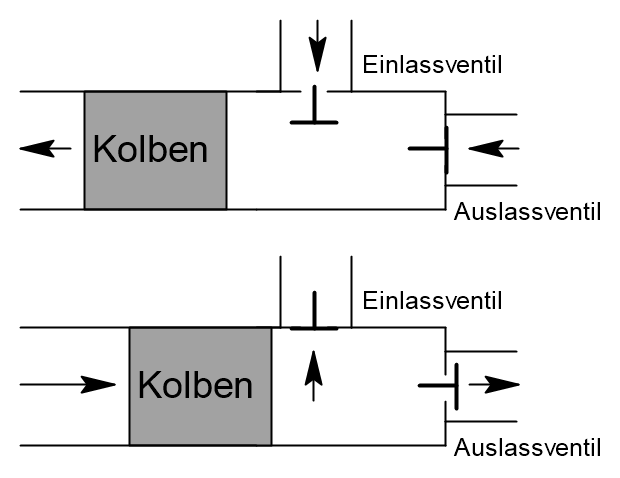
\includegraphics[height=4.25cm]{img/kolbenpumpe}
		\caption{Skizze einer Kolbenpumpe}
		\label{fig:kolbenpumpe}
	\end{minipage}
	%\hspace*{0.05\textwidth}
	\begin{minipage}[b]{0.475\textwidth}
		\centering
		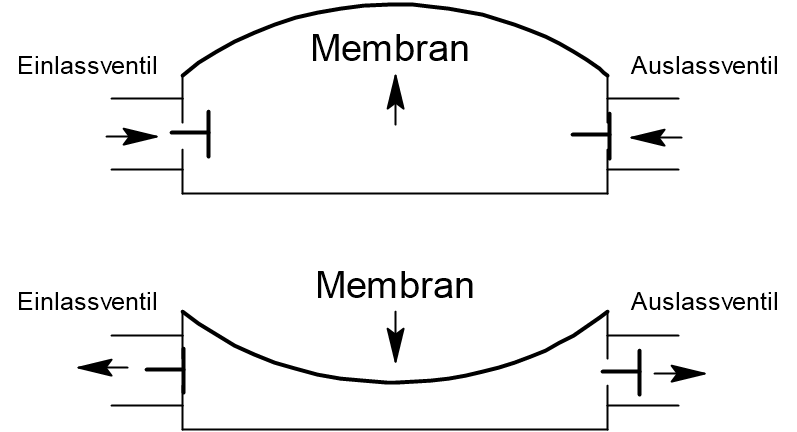
\includegraphics[height=4.25cm]{img/membranpumpe}
		\caption{Skizze einer Membranpumpe}
		\label{fig:membranpumpe}
	\end{minipage}
\end{figure}
\FloatBarrier

Die im Betrieb nutzbaren Stellgrößen bei diesen Pumpen konzentrieren sich aufgrund ihrer Funktionsweise auf die Hublänge und die Hubfrequenz. Durch den geometrisch genau definierten Hubraum und weitestgehend Leckfreien Pumpenventilen und Kolbenabdichtungen, eigenen sich oszillierende Dosierpumpen am günstigsten für die Flüssigkeitsdosierung. Durch das Hubweise fördern der Flüssigkeit ergibt sich jedoch ein digitaler Charakter im Förderstrom. Somit eignen sich diese Pumpen lediglich für diskontinuierliche Dosierung mittels Hubzählung. Der Massenstrom der sich daraus für eine einzylindrige Kolbenpumpe ergibt, ist unter Gleichung \eqref{eq:oz_masse} zu finden. \cite{Vetter.2002}

\begin{equation}
	\label{eq:oz_masse}
	\dot{m} = h_K*A_K*n*\rho*\eta_V
\end{equation}
\begin{parameter}
	\dot{m}		& Fördermassenstrom \\
	h_K			& Hublänge\\
	h_K			& Kolbenquerschnitt\\
	n			& Hubfrequenz\\
	\rho		& Dichte der Flüssigkeit\\
	\eta_V 		& volumetrischer Wirkungsgrad\
\end{parameter}

\paragraph*{Rotierende Verdrängerpumpen} Die Kategorie der rotierenden Dosierpumpen ist im Vergleich zu oszillierenden Dosierpumpen deutlich fassettenreicher. Das hierbei genutzte Verdrängervolumen basiert auf Maßtoleranzen, Spaltmaßen und Elastizitäten des Pumpraumes, welches durch Rotation der Verdrängersystems gefördert wird. Aufgrund dieser Toleranzen treten in rotierenden Verdrängerpumpen für niedrigviskose Flüssigkeiten merkliche, innere Leckagen auf und sind damit weniger genau als oszillierende Verdrängerpumpen. Sie eignen sich daher hauptsächlich für viskose Fluide. Eine Auswahl an typischen, rotierenden Dosierpumpen ist unter Abbildung \ref{fig:rotat_pumpe} dargestellt.

\begin{figure}[h!]
	\centering
	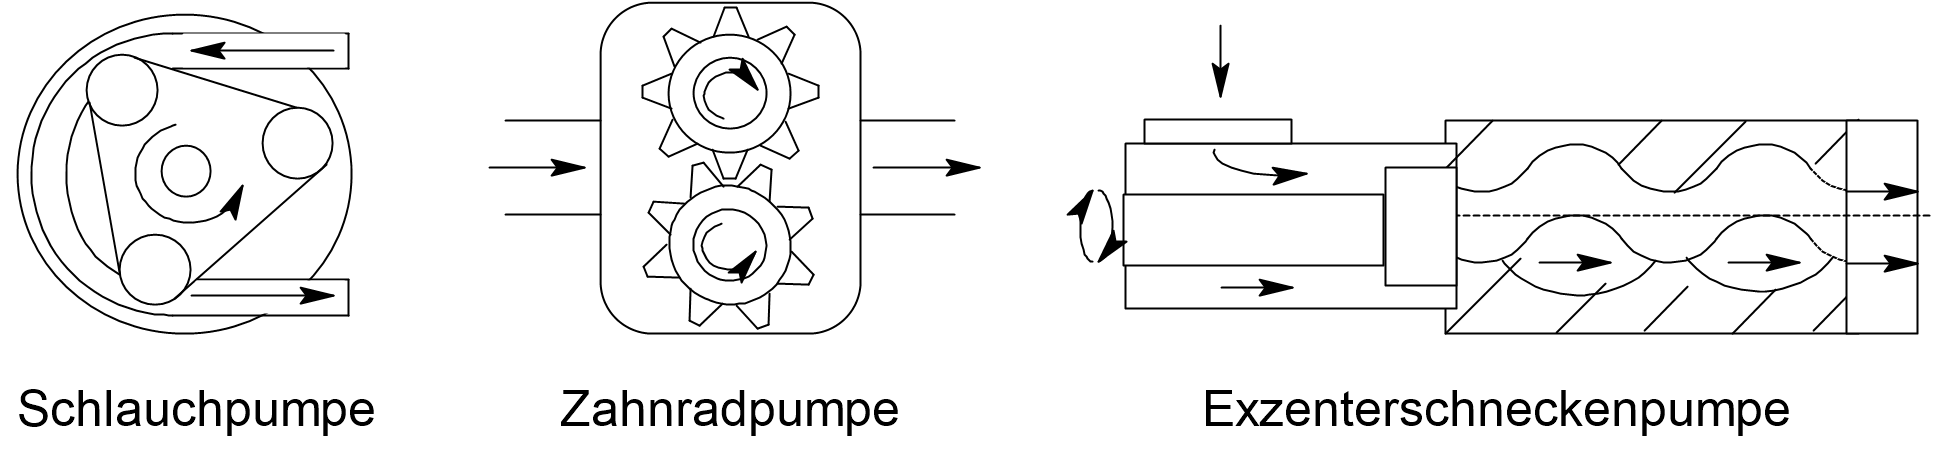
\includegraphics[width=1.0\textwidth]{img/rotationspumpen}
	\caption{Skizzen für Rotationspumpen}
	\label{fig:rotat_pumpe}
\end{figure}
\FloatBarrier

Hauptstellgröße dieser Pumpenart ist die Drehzahl. Ebenso wie bei der Hublänge bzw. der Hubfrequenz oszillierender Verdrängerpumpen besteht bei rotierenden Verdrängerpumpen eine direkte Proportionalität zwischen Drehzahl und Förderstrom. Eine einheitliche Charakteristik des Förderstroms lässt sich für diese Pumpen nicht definieren, da sich trotz Rotationsprinzip die Förderweisen stark unterscheiden. So weisen weißen beispielsweise Schlauchpumpen im Vergleich zu Zahnradpumpen eine viel deutlichere Pulsation des Förderstroms auf, obwohl beide Pumpe den Rotationspumpen zugeordnet werden. Demnach lässt sich auch der Dosierstrom lediglich allgemein wie in Gleichung \eqref{eq:rotations_strom} dargestellt beschreiben. Je nach Pumpentyp lässt sich dann die geometrische Volumenabgrenzung detaillierter ausführen. \cite{Vetter.2002}


\begin{equation}
	\label{eq:rotations_strom}
	\dot{m} = \rho*V_u*n*\eta_V
\end{equation}
\begin{parameter}
	\dot{m}		& Fördermassenstrom \\
	V_u			& Verdrängungsvolumen pro Umdrehung\\
	h_K			& Kolbenquerschnitt\\
	n			& Drehzahl\\
	\rho		& Dichte der Flüssigkeit\\
	\eta_V 		& volumetrischer Wirkungsgrad\
\end{parameter}

Um nach der Vorstellung der verschiedenen Pumpentypen eine Auswahl für die eigene Dosieraufgabe auswählen zu können, sind die verschiedene Kriterien wie Wirkungsgrad, förderbare Viskosität, Druckstabilität, sowie weitere nicht genannte Aspekte heranzuziehen. Einen Überlick hierfür verschafft die Literatur in \mbox{\cite[S. 224 ff.]{Bierwerth.2019}}, sowie ausführlich beschriebene Auswahlhilfen in Form von Tabellen und Diagrammen in \cite[S. 125, 219, 659 ff.]{Vetter.2002}.


\subsubsection{Ermittlung des Dosierstroms}
Je nach Anforderung an die Genauigkeit der Dosierung kommen verschiedene Messsysteme in Frage, um den Dosierstrom zu bestimmen. Hierbei wird zwischen redundanzfreien Dosiersystemen und Dosiersystemen mit Messredundanz unterschieden.\linebreak
Für redundanzfreie Dosiersysteme wird hierbei auf lediglich eine Systemkomponente, wie zum Beispiel der Kennlinie einer Dosierpumpe vertraut, um den geforderten Dosierstrom umzusetzen. Dosiert diese Systemkomponente fehlerhaft bleibt der Fehler unentdeckt. Diese Art der Dosierregelung ist für Prozesse mit geringen Anspruch an Dosiergenauigkeit möglich und deren Konsequenzen im Produktionsprozess tolerierbar sind. In Abbildung \ref{fig:redundanzfrei} ist ein Beispiel für ein redundanzfreies Dosiersystem unter zu Hilfenahme einer Pumpenkennlinie dargestellt.\cite{Vetter.2002}

\begin{figure}[h!]
	\centering
	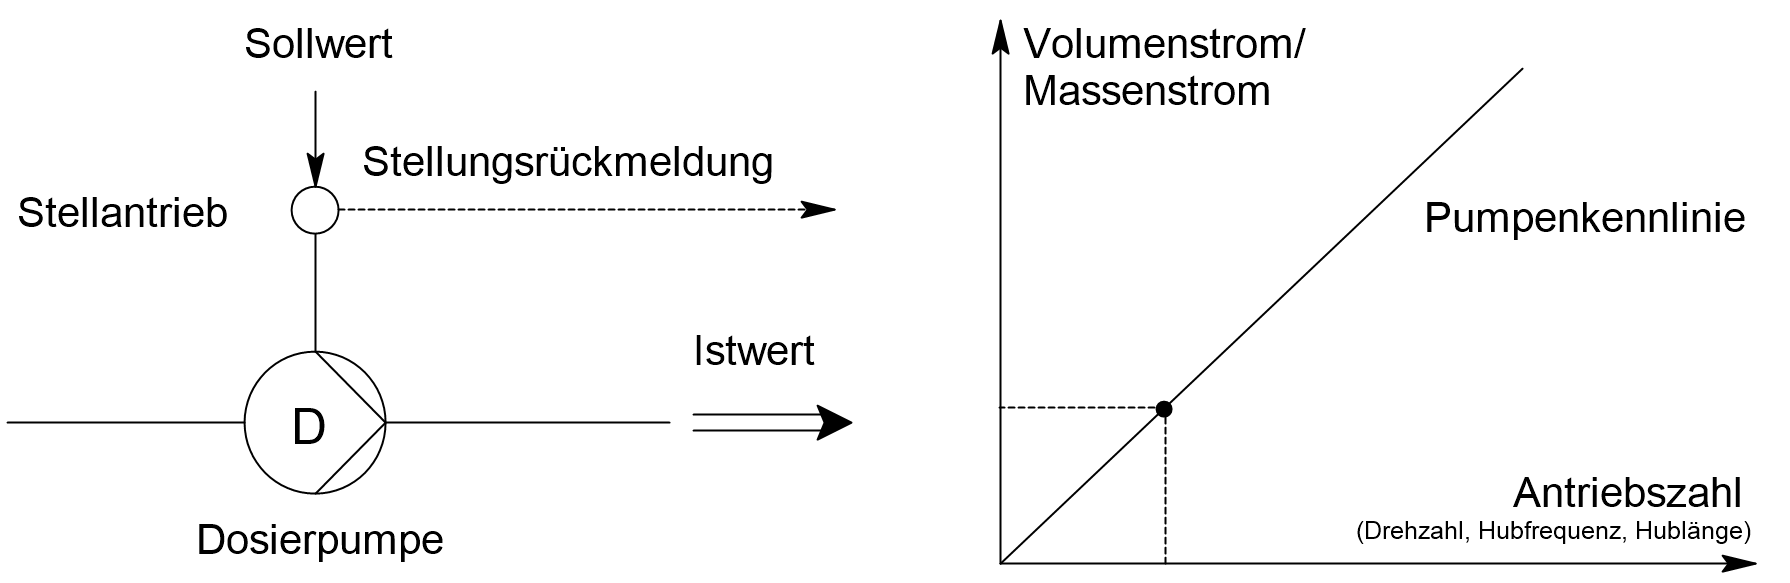
\includegraphics[width=1.0\textwidth]{img/redundanzfrei}
	\caption{Skizze für redundanzfreies Dosiersystem, erstellt nach \cite{Vetter.2002}}
	\label{fig:redundanzfrei}
\end{figure}
\FloatBarrier

In Dosiersystemen mit Messredundanz werden solche Abweichungen durch eine weitere Systemkomponente, wie beispielsweise einem zusätzlichen Durchflussmesser, registriert. Die dadurch geschaffene Fehlervermeidung erhöht die Produktionssicherheit im Prozess, erfordert jedoch auch bereits bei Störung oder Abweichung einer der Komponenten eine Fehlersuche. In Abbildung \ref{fig:redundanz} ist eine beispielhafte Skizze für ein redundant ausgeführtes Dosiersystems mit Dosierpumpe und Durchflussmesser dargestellt.\,\cite{Vetter.2002}

\begin{figure}[h!]
	\centering
	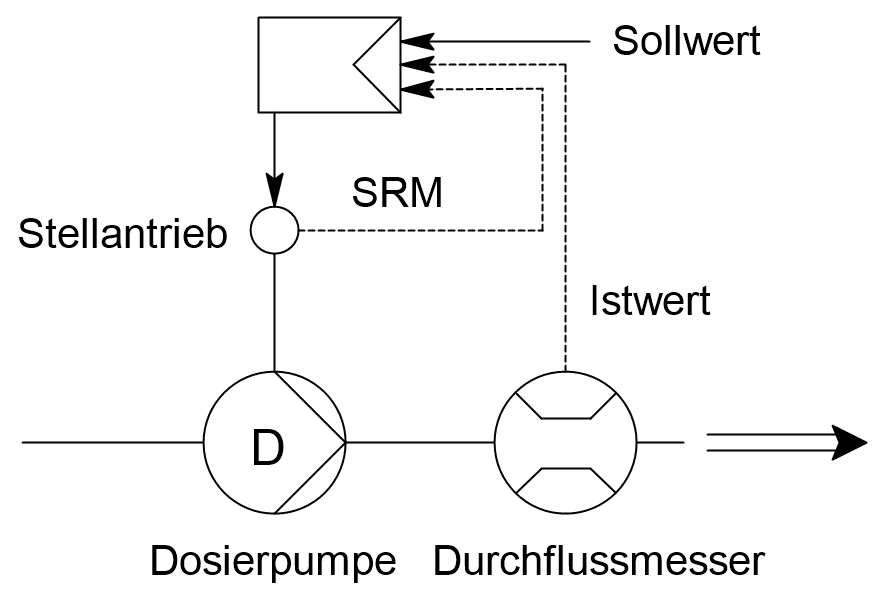
\includegraphics[width=0.5\textwidth]{img/redundanz}
	\caption{Skizze für Dosiersystem mit Redundanz, erstellt nach \cite{Vetter.2002}}
	\label{fig:redundanz}
\end{figure}
\FloatBarrier


Eine Möglichkeit für die redundante Bestimmung des Dosierstroms ist einen Coriolis-Massendurchflussmesser als Systemkomponente zu nutzen. Hierbei wird unter Nutzung einer schwingenden Bewegung, welche auf das strömende Fluid einwirkt, die auftretende Corioliskraft zur Messung des Massenstrom genutzt. Diese wird über induktive Messung der Phasendifferenz zwischen Rohreinlauf und Rohrauslauf bestimmt. Ein Vorteil dieser Art der Durchflussmessung ist, dass neben dem Massenstrom auch Eigenschaften wie die Viskosität, der Massenanteil und die Dichte des Fluides bestimmt werden können. Die Messungen dieser zusätzlichen Parameter basieren dann jedoch auf leicht anderen Messmethoden, als die der Bestimmung des Massenstroms. \cite{Ignatowitz.2015}\linebreak
Nachteil ist jedoch, dass für die Messung nach dem Prinzip der Corioliskraft hohe Strömungsgeschwindigkeiten notwendig sind. Ähnliches gilt übrigens auch für die Messung mittels magnetisch-induktiven Durchflussmesser bei der mindestens ca.\,\SI{0,5}{\meter \per \second} Strömungsgeschwindigkeit notwendig sind. Das kann zum Problem werden, wenn die Strömungsgeschwindigkeit aufgrund von Druckverlusten nicht weiter erhöht werden kann. Das Messverfahren der Ultraschall-Durchflussmessung wäre dann zu den bereits genannten Verfahren eine Alternative, jedoch können durch zu hohe Viskosität des Fluides die erzeugten mechanischen Wellen zu sehr gedämpft werden und es erfolgt keine sinnvolle Messung. \cite{D.Stepanek.Unbekannt, Wikipedia.2021,Wikipedia.2020}\\
Neben den bereits genannten Durchflussmessern gibt es auch so genannte Mengenmesser. Diese beruhen, wenn sie nicht eine Ausführung der zuvor genannten Durchflussmesser sind, meist auf einem Verdrängerprinzip und fungieren als Volumen- oder Geschwindigkeitszähler. Typische Beispiele hierfür sind Ovalradzähler und Turbinenzähler. Speziell Volumenzähler bestimmen die durchgeflossene Menge an Fluid meist durch rotierende Verdrängerkörper wie Zahnräder oder Drehkolben. Durch den Fluss des Fluides drehen sich die Verdrängerkörper und es lassen sich pro Umdrehung die transportierten Volumina des Fluides bestimmen. Vorteil dieser Zähler ist, dass sie meist sehr genau arbeiten und deshalb im Alltag oft als Zähler für Wasser, Benzin  oder Diesel eingesetzt werden. \cite{Ignatowitz.2015}\linebreak
Ihr Nachteil besteht hauptsächlich im mechanischen Wirkprinzip. Dieses hat zur Folge, dass durch zu drehenden Verdrängerkörper für höhere Viskositäten von Fluiden zusätzliche Druckverluste entstehen. Zudem obliegen die Verdrängerkörper durch die mechanische Bewegung oder dem Fluid selbst auch einem gewissen Verschleiß. Zur Bestimmung des Durchflusses ist das gezählte Fördervolumen durch die Förderzeit zusätzlich zu berechnen.\\
Um den Dosierstrom ohne Rohrleitungseinbauten zu bestimmen, ist es möglich ein Loss-in-Weight oder Loss-in-Volume Verfahren zu nutzen. Mit diesen hauptsächlich für schlecht fließende, inhomogene Schüttgüter genutzten Verfahren wird der Massenstrom mittels Differentialdosierer bestimmt. Dieser Differentialdosierer misst den Dosierstrom im klassischen Sinne mit Hilfe einer Waage durch die Gewichtsabnahme über die Zeit. Alternativ ist bei fester, bekannter Geometrie des Dosierbehälters und ausreichender Genauigkeit das selbe Prinzip für eine Füllstands- bzw. Volumenabnahme mit Hilfe eines Radarfüllstandsensors möglich. Vorteil der Förderstrombestimmung über ein solches Loss-in-Weight oder Loss-in-Volume Verfahren liegt darin, dass diese nicht vom Fließverhalten des Mediums beeinflusst werden. Jedoch ist zu bedenken, dass eine ausreichende Auflösung der Messbereiche für die jeweilige Dosierung, sowie der richtige Aufbau für das Messprinzip garantiert werden muss. So ist beispielsweise für die Massenmessung die Entkopplung des Wägesystems und für die Radafüllstandsmessung die einwandfreie Reflexion der Mikrowellensignale an der Dosiergutoberfläche zu gewährleisten. Zudem ist die Dosiergenauigkeit der Radarfüllstandmessung  stark von der Höhe des Dosierbehälters abhängig. Selbst bei $\pm$ \SI{2}{\milli \meter} Messabweichung können diese je nach Behälter bereits mehrere Gramm bis Kilogramm Abweichung bedeuten.\,\cite{Vetter.2002, VEGA.07.02.2022}


%%\paragraph*{Radarfüllstandsmessung}
%%\paragraph*{Gravimetrische Erfassung über Wägezellen}
%
%
%\todo[inline]{Beschreibung der Messprinzipien}


%\subsection{Stand der Technik zur Dosierung hochviskoser Verdickungsmittel}


\subsection{Technische Planung und Dokumentation}
Die technische Planung ist an dieser Stelle als Begriff gewählt worden, da damit ein fachübergreifender Bereich für die Konzeption von Umsetzungsideen umfasst wird. So beinhaltet die Umsetzung einer Dosieranlage nicht nur die Auswahl der Komponenten um das Verfahren umzusetzen, sondern auch die zeichnerische Dokumentation des Verfahrens, sowie Überlegungen der Rohrleitungsauswahl und der zu verarbeitenden Signal sind von entscheidender Bedeutung. 

\subsubsection{R\&I- Fließbild}
Das 

\subsubsection{Rohrleitungsplanung}
\todo[inline]{Rohrklassifizierung und Werkstoff Auswahl ??}


\subsubsection{Signalverarbeitungsplanung}
\todo[inline]{Keine Ahnung selber was ausdenken ?}


%\subsection{Normen und Standards}
%
%
%\subsection{Densimeter}
%
%Norm für Viskositätsbestimmung
%
%https://www.din.de/de/neuer-inhalt/wdc-beuth:din21:306904236
%https://www.din.de/de/wdc-beuth:din21:512291
%https://www.din.de/de/neuer-inhalt/wdc-beuth:din21:329765890
%
%\subsection{Wirtschaftliche Aspekte und Entwicklungsperspektiven}